%
% main.tex -- Paper zum Thema <helmholtz>
%
% (c) 2020 Autor, OST Ostschweizer Fachhochschule
%
% !TEX root = ../../buch.tex
% !TEX encoding = UTF-8
%
\chapter{Helmholtz-Zerlegung\label{chapter:helmholtz}}
\kopflinks{Helmholtz-Zerlegung}
\begin{refsection}
\chapterauthor{Joël Rechsteiner}
\index{Joel Rechsteiner@Joël Rechsteiner}%
\index{Rechsteiner, Joel@Rechsteiner, Joël}%

\noindent
Im Mittelpunkt in diesem Kapitel steht die Helmholtz-Zerlegung.
Anhand eines Beispiels aus der Physik in der Akustik aus dem Paper
\cite{helmholtz:paper}
wird eine Anwendung der Helmholtz-Zerlegung
\index{Helmholtz-Zerlegung}%
dargestellt, wo die komplexe akustischen Intensität in einem
kartesischen Koordinatensystem in wirbelfreie
\index{wirbelfrei}%
und quellenfreie Anteile zerlegt wird.
\index{quellenfrei}%
Allerdings kann die Helmholtz-Zerlegung auch auf ein beliebiges
Koordinatensystem angewendet werden, worauf hier nicht weiter
eingegangen wird.

Schritt für Schritt wird erklärt, wie die relevanten Gleichungen
mit mathematischen Tools vorangegangener Kapitel der Vektoranalysis
mit der physikalischen Deutung zusammenhängen.
Anschliessend wird die Aufteilung der akustischen Intensität in
aktive und reaktive Komponenten aufgezeigt.
\index{aktive Intensitat@aktive Intensität}%
\index{reaktive Intensitat@reaktive Intensität}%
Die Ableitung der Differentialgleichungen für aktive und reaktive
Intensitätsfelder und die Wirbelbildung in der Intensitätsverteilung
zeigen, wie diese Konzepte in numerischen Simulationen wie zum
Beispiel in COMSOL und praktischen Messungen etwa zur Interpretation
\index{COMSOL}%
von Nah- und Fernfeld oder der Quellenkopplung angewendet werden.


%
% teil3.tex -- Beispiel-File für Teil 3
%
% (c) 2020 Prof Dr Andreas Müller, Hochschule Rapperswil
%
% !TEX root = ../../buch.tex
% !TEX encoding = UTF-8
%
\section{Mahtematische Grundlagen
\label{helmholtz:section:Mahtematische_Grundlagen}}
\kopfrechts{Mahtematische Grundlagen}

Hier werden kurz die Tools vorgestellt, welche für die Helmholtz-Zerlegung benötigt werden. Um die Helmholtz-Zerlegung in der Akustik zu verstehen, ist ein solides Verständnis der grundlegenden mathematischen Konzepte notwendig. In diesem Abschnitt werden die wichtigsten Vektoroperatoren und ihre Eigenschaften vorgestellt, die für die Zerlegung von Vektorfeldern benötigt werden.

\subsection{Vektorfelder und Operatoren
\label{helmholtz:subsection:Vektorfelder_Operatoren}}

Vektorfelder stellen in jedem Punkt eines Raumes einen Vektor dar, der sowohl eine Richtung als auch einen Betrag besitzt. In der Akustik sind Vektorfelder von zentraler Bedeutung, da sie physikalische Größen wie die Schallschnelle und die Intensität beschreiben. Um diese Felder zu analysieren, werden spezielle Operatoren verwendet, die lokale Eigenschaften des Feldes charakterisieren.

\subsubsection{Der Gradient eines Skalarfeldes}

Der Gradient eines Skalarfeldes $a$ ist ein Vektorfeld, das in jedem Punkt in Richtung des steilsten Anstiegs von $a$ zeigt. Mathematisch wird der Gradient durch folgende Gleichung definiert:

\begin{equation}
\mathbf{\nabla} a (\mathbf{r}) = \frac{\partial a}{\partial x}\mathbf{e}_x + \frac{\partial a}{\partial y}\mathbf{e}_y + \frac{\partial a}{\partial z}\mathbf{e}_z
\end{equation}

Der Gradient wirkt auf ein Skalarfeld und liefert ein Vektorfeld, das in Richtung des steilsten Anstiegs von $a$ zeigt. Der Gradient an einem Punkt ergibt die Richtung maximaler Zunahme des Skalars, während sein Betrag der Steigung in der entsprechenden Richtung entspricht.

\subsubsection{Die Divergenz eines Vektorfeldes}

Die Divergenz eines Vektorfeldes $\mathbf{F}$ ist ein Skalarfeld, das beschreibt, wie stark Feldlinien auseinanderstreben oder zusammenlaufen. Sie wird durch folgende Formel ausgedrückt

\begin{equation}
\nabla \cdot \mathbf{F}(\mathbf{r}) = \frac{\partial F_x}{\partial x} + \frac{\partial F_y}{\partial y} + \frac{\partial F_z}{\partial z}.
\end{equation}

\noindent Die Divergenz kann als Mass für die Quellen- oder Senken-stärke an einem bestimmten Punkt im Vektorfeld interpretiert werden. Ein Bereich mit positiver Divergenz stellt eine Quelle dar, aus der Feldlinien hervorgehen, während ein Bereich mit negativer Divergenz eine Senke darstellt, in der Feldlinien zusammenlaufen, wie in Abbildung \ref{fig:DivergenzAlg} dargestellt.

\begin{figure}[h!]
    \centering
    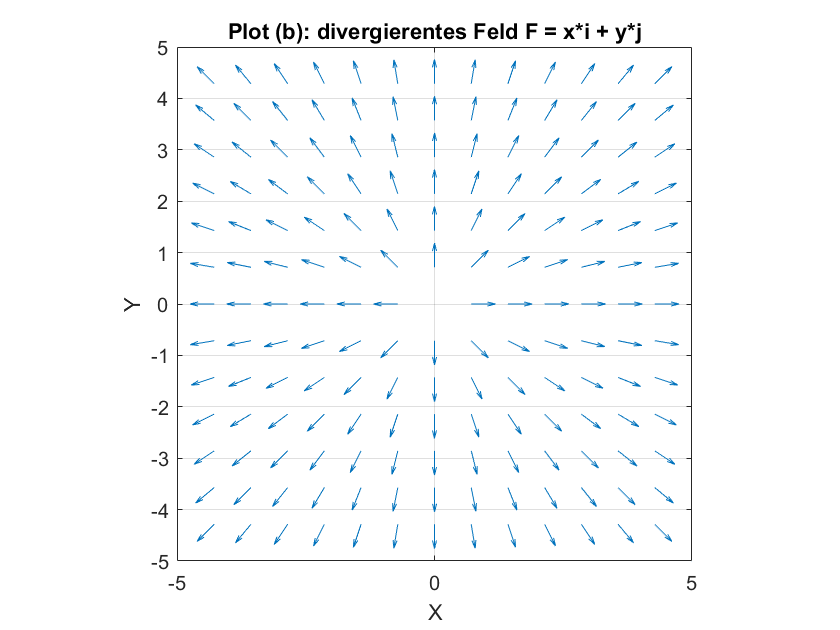
\includegraphics[scale=0.4]{papers/helmholtz/images/divergentes_Feld.png}
    \caption{Beispiel eines divergenten Vektorfeldes, das Quellen und Senken aufweist}
    \label{fig:DivergenzAlg}
\end{figure}

\subsubsection{Die Rotation eines Vektorfeldes}

Die Rotation eines Vektorfeldes $\mathbf{A}$ ist ein Vektorfeld, das die Wirbeldichte des ursprünglichen Feldes beschreibt. Sie wird definiert als

\begin{equation}
\nabla \times \mathbf{A}(\mathbf{r}) = \begin{vmatrix}
    \mathbf{e}_x & \mathbf{e}_y & \mathbf{e}_z \\
    \frac{\partial}{\partial x} & \frac{\partial}{\partial y} & \frac{\partial}{\partial z}\\
    A_x & A_y & A_z
\end{vmatrix}.
\end{equation}

\noindent Die Rotation misst, wie stark sich die Feldlinien um eine Achse drehen und gibt sowohl die Achsenorientierung als auch die Stärke eines solchen Wirbels an, wie in Abbildung \ref{fig:RotationAlg} zu sehen ist.

\begin{figure}[h!]
    \centering
    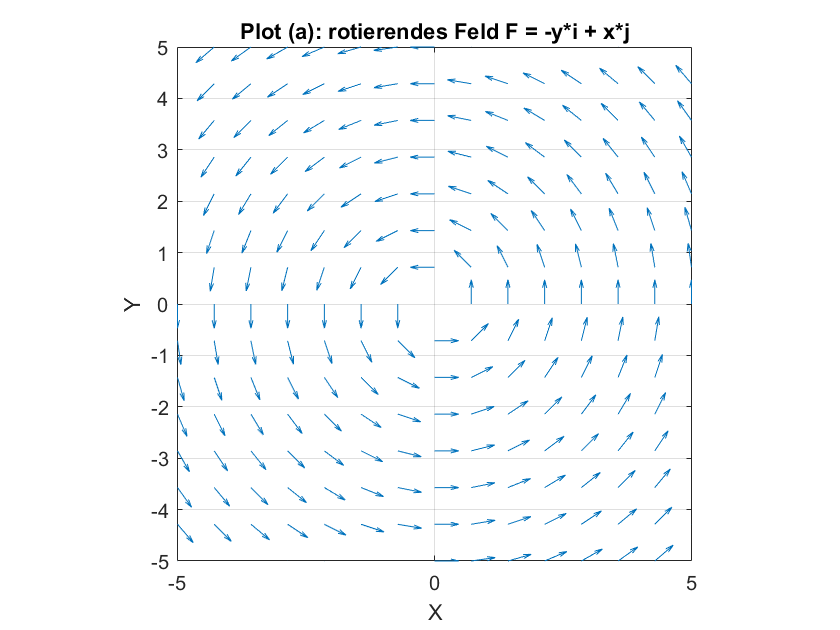
\includegraphics[scale=0.4]{papers/helmholtz/images/rotierendes_Feld.png}
    \caption{Beispiel eines rotierenden Vektorfeldes mit deutlich erkennbarer Wirbelstruktur}
    \label{fig:RotationAlg}
\end{figure}

\subsubsection{Der Laplace-Operator}

Der Laplace-Operator, oft als $\nabla^2$ oder $\Delta$ geschrieben, ist ein skalarer Differentialoperator zweiter Ordnung. Angewendet auf ein Skalarfeld $a$ ergibt er

\begin{equation}
\nabla^2 a(\mathbf{r}) = \frac{\partial^2 a}{\partial x^2} + \frac{\partial^2 a}{\partial y^2} + \frac{\partial^2 a}{\partial z^2}.
\end{equation}

Der Laplace-Operator spielt eine zentrale Rolle in vielen physikalischen Gleichungen, insbesondere in der Potentialtheorie und der Wellenausbreitung. Für ein Vektorfeld $\mathbf{F}$ wird der Laplace-Operator komponentenweise angewendet und das Resultat kann wie in \ref{fig:LaplaceAlg} dargestellt aussehen. Die Formel für den Laplace-Operation ist

\begin{equation}
\nabla^2 \mathbf{F} = (\nabla^2 F_x)\mathbf{e}_x + (\nabla^2 F_y)\mathbf{e}_y + (\nabla^2 F_z)\mathbf{e}_z.
\end{equation}

\begin{figure}[h!]
    \centering
    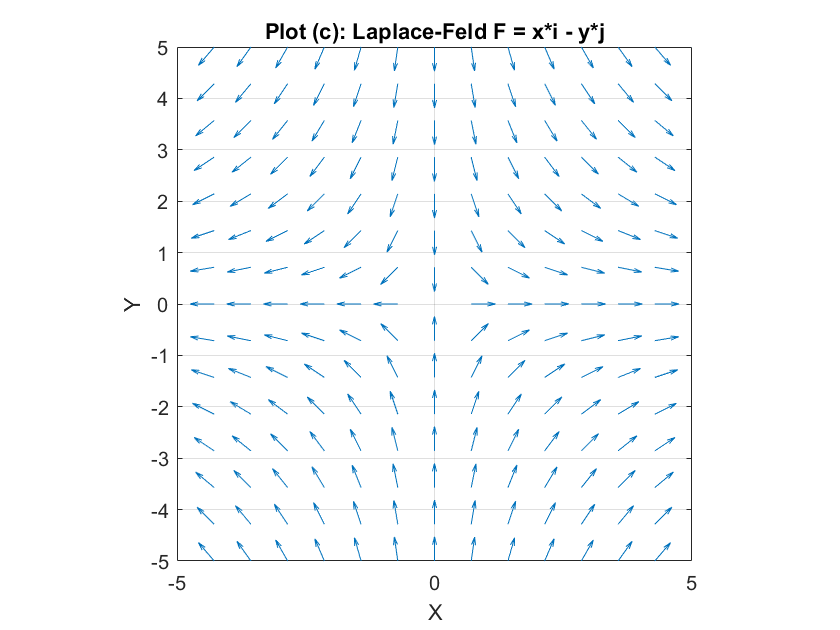
\includegraphics[scale=0.4]{papers/helmholtz/images/Laplace_Feld.png}
    \caption{Visualisierung des Laplace-Operators auf ein Skalarfeld}
    \label{fig:LaplaceAlg}
\end{figure}


\subsection{Vektoridentitäten
\label{helmholtz:subsection:Vektoridentitaeten}}
Für die mathematische Herleitung der Helmholtz-Zerlegung werden verschiedene Vektoridentitäten benötigt.

\subsubsection{Wichtige Vektoridentitäten}

Die folgenden Identitäten sind für die Ableitung der Helmholtz-Zerlegung besonders relevant:

\begin{itemize}
\item Für jedes Skalarfeld $\Phi$ gilt: $\nabla \times (\nabla \Phi) = 0$
\item Für jedes Vektorfeld $\mathbf{F}$ gilt: $\nabla \cdot (\nabla \times \mathbf{F}) = 0$
\item Der Laplace-Operator eines Vektorfeldes lässt sich umformen zu:
\begin{equation}
\nabla^2 \mathbf{F} = \nabla(\nabla \cdot \mathbf{F}) - \nabla \times (\nabla \times \mathbf{F})
\end{equation}
\noindent Diese Identität ist fundamental für die Ableitung der Helmholtz-Zerlegung.
\end{itemize}





%
% teil3.tex -- Beispiel-File für Teil 3
%
% (c) 2020 Prof Dr Andreas Müller, Hochschule Rapperswil
%
% !TEX root = ../../buch.tex
% !TEX encoding = UTF-8
%
\section{Die Helmholtz-Zerlegung
\label{helmholtz:section:Helmholtz_Zerlegung}}
\kopfrechts{Helmholtz-Zerlegung}

Die Grundidee der Helmholtz-Zerlegung besteht darin, dass ein differenzierbares  Vektorfeld $\boldsymbol{F}$, welches im Unendlichen schnell genug abfällt, sich in zwei in noch zu spezifizierendem Sinne orthogonale Komponenten zerlegen lässt: einen eindeutig wirbelfreien Teil und einen quellenfreien Teil. Diese Zerlegung spiegelt die physikalischen Eigenschaften des Vektorfeldes wider und ist insbesondere in der Akustik, Strömungsmechanik und Elektrodynamik von zentraler Bedeutung.

\subsection{Formale Definition der Helmholtz-Zerlegung
\label{helmholtz:subsection:def_Helmholtz_Zerlegung}}

Mit der Idee der Helmholtz-Zerlegung wird das Vektorfeld geschrieben als
\begin{equation}
\underbrace{\boldsymbol{F}}_{\text{zu zerlegendes Vektorfeld}} = \underbrace{-\nabla \Phi}_{\text{irrotationaler Teil}} + \underbrace{\nabla \times \boldsymbol{\Psi}}_{\text{solenoidaler Teil}} 
\label{helmholtz:equationAllgemein}
\end{equation}
und die einzelnen Komponenten lässt sich wie folgt beschreiben:

\begin{itemize}
\item Der erste Term $ -\nabla \Phi $ ist wirbelfrei, da seine Rotation verschwindet.
\begin{itemize}
\item Dieser Anteil hat keine Rotation: $\nabla \times (-\nabla \Phi) = 0$.
\item Die Feldlinien verlaufen strahlenförmig von Quellen zu Senken.
\end{itemize}

\item Der zweite Term $\nabla \times \boldsymbol{\Psi}$ hat gemäss der Definition immer Divergenz gleich null und wird auch solenoidal genannt.
\begin{itemize}
\item Dieser Anteil hat keine Divergenz: $\nabla \cdot (\nabla \times \boldsymbol{\Psi}) = 0$.
\item Die Feldlinien bilden geschlossene Schleifen ähnlich einem Magnetfeld.
\end{itemize}
\end{itemize}

\begin{table}
\centering
\begin{tabular}{l|l|l|l}
\hline
Komponente & Potential & Eigenschaft & Bezeichnung \\
\hline 
Irrotationaler Teil & $\Phi$ (Skalarpotential) & $\nabla \times (-\nabla \Phi) = 0$ & wirbelfrei\\
Solenoidaler Teil & $\boldsymbol{\Psi}$ (Vektorpotential) & $\nabla \cdot (\nabla \times \boldsymbol{\Psi}) = 0$ & quellenfrei\\
\hline
\end{tabular}
\caption{Übersicht der Helmholtz-Zerlegung}
\label{tab:helmholtz_overview}
\end{table}

In der Tabelle \ref{tab:helmholtz_overview} ist die komplementäre Eigeschaft, die Bezeichnung und die Potentialbeschreibung der jeqeiligen Komponenten zusammengefasst.

Um die Zerlegung anwenden zu können, müssen die Potentiale $\Phi$ und $\boldsymbol{\Psi}$ berechnet werden. Dies kann auf verschiedene Weisen erfolgen, abhängig von den Randbedingungen.

\subsection{Mathematischer Nachweis der Eigenschaften
\label{helmholtz:subsection:math_Nachweis}}

\subsubsection{Nachweis der Wirbelfreiheit des irrotationalen Anteils}
Sei $\Phi$ ein zweimal stetig differenzierbares Skalarfeld.

\begin{enumerate}
    \item Zuerst wird der Gradient $\nabla\Phi$ berechnet:
    Der Gradient ergibt
    \[
    \nabla \Phi =
	\renewcommand{\arraystretch}{2.0}
    \begin{pmatrix}
        \displaystyle \frac{\partial \Phi}{\partial x} \\
        \displaystyle \frac{\partial \Phi}{\partial y} \\
        \displaystyle \frac{\partial \Phi}{\partial z}
    \end{pmatrix}.
    \]

    \item Nun die Rotation dieses Gradientenfeldes: Die Definitionsformel der Rotation $\nabla \times \boldsymbol{F}$ auf den Gradientenvektor anwenden ergibt
    \[
    \nabla \times (\nabla \Phi) =
	\renewcommand{\arraystretch}{2.0}
    \begin{pmatrix}
        \displaystyle\frac{\partial}{\partial y}\left(\frac{\partial \Phi}{\partial z}\right) - \frac{\partial}{\partial z}\left(\frac{\partial \Phi}{\partial y}\right) \\
        \displaystyle\frac{\partial}{\partial z}\left(\frac{\partial \Phi}{\partial x}\right) - \frac{\partial}{\partial x}\left(\frac{\partial \Phi}{\partial z}\right) \\
        \displaystyle\frac{\partial}{\partial x}\left(\frac{\partial \Phi}{\partial y}\right) - \frac{\partial}{\partial y}\left(\frac{\partial \Phi}{\partial x}\right)
    \end{pmatrix}.
    \]

    \item %Den \emph{Satz von Schwarz} anwenden:
    
    Zur besseren Übersicht werden die gemischten Ableitungen ausgeschrieben:
    \[
    \nabla \times (\nabla \Phi) =
	\renewcommand{\arraystretch}{2.0}
    \begin{pmatrix}
        \displaystyle\frac{\partial^2 \Phi}{\partial y\, \partial z} - \frac{\partial^2 \Phi}{\partial z\, \partial y} \\
        \displaystyle\frac{\partial^2 \Phi}{\partial z\, \partial x} - \frac{\partial^2 \Phi}{\partial x\, \partial z} \\
        \displaystyle\frac{\partial^2 \Phi}{\partial x\, \partial y} - \frac{\partial^2 \Phi}{\partial y\, \partial x}
    \end{pmatrix}.
    \]
    Der \emph{Satz von Schwarz} besagt, dass bei stetigen differenzierbaren
    Funktionen die Reihenfolge der partiellen Ableitungen vertauscht werden
    kann.
    Damit heben sich die Terme in jeder Komponente gegenseitig auf und es bleibt
    \[
    \nabla \times (\nabla \Phi)  =
    \begin{pmatrix}
        0 \\
        0 \\
        0
    \end{pmatrix} = \boldsymbol{0}.
    \]
\end{enumerate}

\subsubsection{Nachweis der Quellenfreiheit des solenoidalen Anteils}

\begin{enumerate}
    \item Berechnung der Rotation $\nabla \times \boldsymbol{\Psi}$:
	Zuerst wird der Rotations-Operator auf $\boldsymbol{\Psi}$ angewendet:
    \[
    \nabla \times \boldsymbol{\Psi} =
	\renewcommand{\arraystretch}{2.0}
    \begin{pmatrix}
        \displaystyle\frac{\partial \Psi_z}{\partial y} - \frac{\partial \Psi_y}{\partial z} \\
        \displaystyle\frac{\partial \Psi_x}{\partial z} - \frac{\partial \Psi_z}{\partial x} \\
        \displaystyle\frac{\partial \Psi_y}{\partial x} - \frac{\partial \Psi_x}{\partial y}
    \end{pmatrix}.
    \]

    \item Berechnung der Divergenz des Ergebnisses: Nun wird der Divergenz-Operator auf das resultierende Vektorfeld angewendet. Dies geschieht durch die Summe der partiellen Ableitungen der Komponenten nach der jeweiligen Koordinate.
    
    \begin{align*}
    % Schritt 1: Definition der Divergenz anwenden
    \nabla \cdot (\nabla \times \boldsymbol{\Psi}) &= \frac{\partial}{\partial x}\left( \frac{\partial \Psi_z}{\partial y} - \frac{\partial \Psi_y}{\partial z} \right) + \frac{\partial}{\partial y}\left( \frac{\partial \Psi_x}{\partial z} - \frac{\partial \Psi_z}{\partial x} \right) + \frac{\partial}{\partial z}\left( \frac{\partial \Psi_y}{\partial x} - \frac{\partial \Psi_x}{\partial y} \right) \\
    % Schritt 2: Die Ableitungen ausführen
    &= \frac{\partial^2 \Psi_z}{\partial x\, \partial y} - \frac{\partial^2 \Psi_y}{\partial x\, \partial z} + \frac{\partial^2 \Psi_x}{\partial y\, \partial z} - \frac{\partial^2 \Psi_z}{\partial y\, \partial x} + \frac{\partial^2 \Psi_y}{\partial z\, \partial x} - \frac{\partial^2 \Psi_x}{\partial z\, \partial y} \\
    % Schritt 3: Terme umsortieren, um Paare zu bilden
    &= \left( \frac{\partial^2 \Psi_x}{\partial y\, \partial z} - \frac{\partial^2 \Psi_x}{\partial z\, \partial y} \right) + \left( \frac{\partial^2 \Psi_y}{\partial z\, \partial x} - \frac{\partial^2 \Psi_y}{\partial x\, \partial z} \right) + \left( \frac{\partial^2 \Psi_z}{\partial x\, \partial y} - \frac{\partial^2 \Psi_z}{\partial y\, \partial x} \right) = 0.
    \end{align*}
    
    \item Nach dem \emph{Satz von Schwarz} ist die Reihenfolge der partiellen Ableitungen bei zweimal stetig differenzierbaren Funktionen irrelevant. Daher gilt:
    \[
    \frac{\partial^2 f}{\partial x\, \partial y} = \frac{\partial^2 f}{\partial y\, \partial x}.
    \]
    Angewendet auf die obige Gleichung bedeutet dies, dass jeder Term in den Klammern Null ergibt:
    \begin{align*}
    \nabla \cdot (\nabla \times \boldsymbol{\Psi})
&=
\underbrace{\left( \frac{\partial^2 \Psi_x}{\partial y\, \partial z} - \frac{\partial^2 \Psi_x}{\partial y\, \partial z} \right)}_{\displaystyle=0}
+
\underbrace{\left( \frac{\partial^2 \Psi_y}{\partial z\, \partial x} - \frac{\partial^2 \Psi_y}{\partial z\, \partial x} \right)}_{\displaystyle=0}
+
\underbrace{\left( \frac{\partial^2 \Psi_z}{\partial x\, \partial y} - \frac{\partial^2 \Psi_z}{\partial x\, \partial y} \right)}_{\displaystyle=0} \\
    &= 0 + 0 + 0 \\
    &= 0.
    \end{align*}
\end{enumerate}
Damit ist die Identität $\nabla \cdot (\nabla \times \boldsymbol{\Psi}) = 0$ bewiesen.


\subsection{Berechnung der Potentiale
\label{helmholtz:subsection:Berechnung der Potentiale}}

\subsubsection{Greenscher Ansatz}
Ein möglicher Ansatz zur Lösung der partiellen Differentialgleichung
ist die Verwendung der Dirac-Delta-Funktion und des greenschen
Funktionen wie dies in \cite{baird_helmholtz} beschrieben ist.
Dies entspricht der Integralform einer Matrixmultiplikation, wie
in Tabelle \ref{tab:helmholtz_matrix_analogie} veranschaulicht.
Dabei wird die Funktion $\boldsymbol{F}$, die in diesem Fall einen
Vektor darstellt, mit der Delta-Funktion multipliziert wie folgt:

\begin{equation}
\Delta F = -4 \pi \rho. 
\label{helmholtz:DGL_idee}
\end{equation}

\begin{equation}
\underbrace{\frac{1}{4 \pi} \Delta F}_{\text{invertiert}} = \rho 
\label{helmholtz:DGL_idee_umformung}
\end{equation}

\begin{table}
\centering
\begin{tabular}{l|l}
  & Idee in Matrixnotation \\
\hline
$\Delta F = -4 \pi \rho$  & $Au = f$ \\
$\underbrace{\frac{1}{4 \pi} \Delta F}_{invertiert} = \rho$ & $A^{-1}Au = A^{-1}f$  \\
 & $u = A^{-1}f$  \\
 \hline
\end{tabular}
\caption{Analogie zur Matrixinversion}
\label{tab:helmholtz_matrix_analogie}
\end{table}

Grundlegend für diesen Ansatz ist die Beziehung
\begin{equation}
\delta (\boldsymbol{x} - \boldsymbol{x'}) = \frac{1}{4 \pi} \nabla^2 \frac{1}{|\boldsymbol{x} - \boldsymbol{x'}|}.
\label{helmholtz:dirac}
\end{equation}
Diese Beziehung lässt sich analog zur Multiplikation mit der Einheitsmatrix verstehen, was es ermöglicht, das Vektorfeld $\boldsymbol{F}$ durch das Volumenintegral
\begin{equation}
\boldsymbol{F}(\boldsymbol{r}) = -\frac{1}{4\pi} \int_V \boldsymbol{F}(\boldsymbol{r}') \nabla^2 \left( \frac{1}{|\boldsymbol{r} - \boldsymbol{r}'|} \right) dV'
\end{equation}
auszudrücken.

Unter Verwendung der Vektoridentität
\begin{equation}
\nabla^2 \boldsymbol{\Psi}= \underbrace{\nabla \Big( \nabla \cdot \boldsymbol{\Psi} \Big)}_{\text{Gradient}} -\underbrace{\nabla \times \Big(\nabla \times \boldsymbol{\Psi} \Big)}_{\text{Rotation}},
\end{equation}
kann das Vektorfeld $\boldsymbol{F}$ geschrieben werden als:
\begin{equation}
\boldsymbol{F}(\boldsymbol{r}) = - \frac{1}{4 \pi} \nabla ( \nabla \cdot \int_V \frac{\boldsymbol{F}(\boldsymbol{x}^{\prime})}{|\boldsymbol{r} - \boldsymbol{r}^{\prime}|} d\boldsymbol{x}^{\prime} ) + \frac{1}{4 \pi} \nabla \times ( \nabla \times \int_V \frac{\boldsymbol{F}(\boldsymbol{x}^{\prime})}{|\boldsymbol{r} - \boldsymbol{r}^{\prime}|} d\boldsymbol{x}^{\prime} ).
\end{equation}
Diese Gleichung repräsentiert die Helmholtz-Zerlegung des Vektorfeldes $\boldsymbol{F}$.

\subsubsection{Berechnung der Potentiale in unbeschränkten Gebieten}

Die Potentiale $\Phi$ und $\boldsymbol{\Psi}$ lassen sich für unbeschränkte Gebiete mit Hilfe der greenschen Funktion wie folgt berechnen:

\begin{itemize}
\item Skalares Potential:
\begin{equation}
\Phi(\boldsymbol{r}) = \frac{1}{4 \pi} \int_{V} \frac{\nabla' \cdot \boldsymbol{F}(\boldsymbol{r'})}{|\boldsymbol{r} - \boldsymbol{r'}|} dV'.
\end{equation}

\item Vektorpotential:
\begin{equation}
\boldsymbol{\Psi}(\boldsymbol{r}) = \frac{1}{4 \pi} \int_{V} \frac{\nabla' \times \boldsymbol{F}(\boldsymbol{r'})}{|\boldsymbol{r} - \boldsymbol{r'}|} dV'.
\end{equation}
\end{itemize}
Hier bezeichnet $\nabla'$ den Nabla-Operator bezüglich der Integrationsvariablen $\boldsymbol{r'}$.

\subsubsection{Berechnung der Potentiale in beschränkten Gebieten}

Für endliche Volumina $V$ mit Oberfläche $S$ müssen zusätzliche Oberflächenintegrale berücksichtigt werden:

\begin{itemize}
\item Skalares Potential:
\begin{equation}
\Phi (\boldsymbol{r}) = \frac{1}{4\pi} \int_V \frac{\nabla' \cdot \boldsymbol{F}(\boldsymbol{r}')}{|\boldsymbol{r} - \boldsymbol{r}'|} dV' + \frac{1}{4\pi} \oint_S \frac{\boldsymbol{F}(\boldsymbol{r}') \cdot \boldsymbol{n}}{|\boldsymbol{r} - \boldsymbol{r}'|} dS'
\end{equation}

\item Vektorpotential:
\begin{equation}
\boldsymbol{\Psi}(\boldsymbol{r}) = \frac{1}{4\pi} \int_V \frac{\nabla' \times \boldsymbol{F}(\boldsymbol{r}')}{|\boldsymbol{r} - \boldsymbol{r}'|} dV' + \frac{1}{4\pi} \oint_S \frac{\boldsymbol{n} \times \boldsymbol{F}(\boldsymbol{r}')}{|\boldsymbol{r} - \boldsymbol{r}'|} dS'
\end{equation}
\end{itemize}
Hier bezeichnet $\boldsymbol{n}$ den nach aussen gerichteten Normalenvektor auf der Oberfläche $S$.

\subsection{Bedingungen und Eindeutigkeit
\label{helmholtz:subsection:Bedingungen_Eindeutigkeit}}

\subsubsection{Voraussetzungen für die Anwendbarkeit}
Damit die Zerlegung korrekt durchgeführt werden kann, muss das Vektorfeld $\boldsymbol{F}$ folgende Bedingungen erfüllen:

\begin{itemize}
\item Glattheit: $\boldsymbol{F}$ muss stetig differenzierbar sein in dem betrachteten Gebiet.
\item Abfallverhalten: $\boldsymbol{F}$ muss im Unendlichen schneller als $\frac{1}{r}$ abfallen, d.h.
\begin{equation}
\lim_{r \to \infty} r|\boldsymbol{F}(\boldsymbol{r})| = 0,
\end{equation}
wobei $r = |\boldsymbol{r}|$ der Abstand vom Ursprung ist.
\end{itemize}
Diese Bedingungen stellen sicher, dass die Integrale in der greenschen
Formulierung konvergieren und die Zerlegung eindeutig ist.

\subsubsection{Eindeutigkeit der Zerlegung
\label{helmholtz:subsection:Bedingungen_onlyEindeutigkeit}}

Die Eindeutigkeit der Helmholtz-Zerlegung hängt von den Randbedingungen ab:

\begin{itemize}
\item Für unbeschränkte Gebiete: Die Zerlegung ist eindeutig, wenn
das Vektorfeld im Unendlichen gegen null geht.
Diese Bedingung stellt sicher, dass bestimmte Oberflächenintegrale
bei der Herleitung der Zerlegung verschwinden \cite{wiki:helmholtz}.

\item Für beschränkte Gebiete: Die Eindeutigkeit erfordert zusätzliche Randbedingungen.
Obwohl das Vektorfeld auch als Summe eines irrotationalen und eines
solenoidalen Anteils geschrieben werden kann, ist für eine eindeutige
Lösung die Festlegung von Randbedingungen notwendig \cite{wiki:helmholtz}.
Typischerweise sind dies:
  \begin{itemize}
    \item Festlegung der Normalkomponente des irrotationalen Teils auf dem Rand.
    \item Festlegung der Tangentialkomponente des solenoidalen Teils auf dem Rand.
  \end{itemize}
\end{itemize}

\subsubsection{Orthogonalität der Komponenten}

Eine wichtige Eigenschaft der Helmholtz-Zerlegung ist die Orthogonalität der beiden Komponenten.
Für ein Vektorfeld $\boldsymbol{F} = \boldsymbol{F}_{\text{irr}} + \boldsymbol{F}_{\text{sol}}$ gilt unter geeigneten Randbedingungen:
\begin{equation}
\int_V \boldsymbol{F}_{\text{irr}} \cdot \boldsymbol{F}_{\text{sol}} \, dV = 0.
\end{equation}
%
% XXX Inkorrekter Satz
%
Das Integral ist null, weil es mithilfe des Gaussschen Integralsatzes
in ein Oberflächenintegral umgewandelt werden kann, das unter den
für die Helmholtz-Zerlegung Randbedingungen, wie in
\ref{helmholtz:subsection:Bedingungen_onlyEindeutigkeit} beschrieben,
verschwindet.
 
In physikalischen Anwendungen, wie beispielsweise in der Akustik,
bedeutet diese mathematische Orthogonalität, dass die beiden
Feldkomponenten unterschiedliche physikalische Phänomene beschreiben,
die unabhängig voneinander analysiert werden können.
Mehr dazu wird im Abschnitt~\ref{tab:helmholtz:Energie_Interpretation}
erläutert.



%
% teil3.tex -- Beispiel-File für Teil 3
%
% (c) 2020 Prof Dr Andreas Müller, Hochschule Rapperswil
%
% !TEX root = ../../buch.tex
% !TEX encoding = UTF-8
%
\section{Akustische Grundlagen und Feldtheorie
\label{helmholtz:section:akustische_Grundlagen}}
\kopfrechts{Akustische Grundlagen und Feldtheorie}

Um die Anwendung der Helmholtz-Zerlegung in der Akustik zu verstehen, bedarf es grundlegender Kenntnisse der physikalischen Akustik.
Hier werden die zentralen physikalischen Grössen Schalldruck, Schallschnelle und deren Zusammenhänge erläutert.
In vielen akustischen Aufgaben wird mit der komplexen Schreibweise gearbeitet, weshalb die Formeln vorzugsweise im Frequenzbereich dargestellt werden.

\subsubsection{Die komplexe Schreibweise in der Akustik}

In der physikalischen Akustik wird häufig mit komplexen Grössen gearbeitet, bei denen der Imaginärteil eine konkrete physikalische Bedeutung hat. Diese mathematische Darstellung ist nicht nur ein Rechentrick, sondern erlaubt eine präzise Beschreibung von Phasenbeziehungen zwischen akustischen Grössen:

\begin{itemize}
\item Der Realteil einer komplexen akustischen Grösse entspricht der tatsächlichen, messbaren physikalischen Grösse zu einem bestimmten Zeitpunkt.

\item Der Imaginärteil repräsentiert die um 90° phasenverschobene Komponente und beschreibt somit zeitliche Verzögerungen im harmonischen Schwingungsverhalten.
\end{itemize}
Diese komplexe Darstellung hat besondere Bedeutung für die Energiebetrachtung in akustischen Feldern worauf später noch genauer beschrieben wird.

Die physikalische Interpretation der komplexen Grössen wird besonders deutlich bei der Betrachtung der komplexen Schallintensität, wo der Realteil die aktive und der Imaginärteil die reaktive Energiekomponente beschreibt \cite{helmholtz:paper}.



\subsection{Grundbegriffe der physikalischen Akustik
\label{helmholtz:subsection:Grundbegriffe_Akustik}}

\subsubsection{Schalldruck $p$}
 
Der Schalldruck ist eine der fundamentalen Größen in der Akustik und beschreibt lokale Druckschwankungen im Medium:
 
\begin{itemize}
\item $P  (\boldsymbol{r})$ bezeichnet die Amplitude des Schalldrucks am Ort $\boldsymbol{r}$ und ist eine reelle Grösse.
\item $\omega$ ist die Kreisfrequenz.
\item $\phi  (\boldsymbol{r})$ beschreibt die Phase am Ort $\boldsymbol{r}$ und ist ebenfalls eine reelle Grösse.
\end{itemize}
 
Die zeitabhängige Darstellung des Schalldrucks lautet:
\begin{equation}
p(r,t) = P(\boldsymbol{r})  e^{j( \omega t - \phi(\boldsymbol{r}))} (\si{\pascal}).
\end{equation}
 
Im Frequenzbereich, auch Phasor-Darstellung genannt, bei einer festen Frequenz $\omega$ vereinfacht sich dies zu:
\begin{equation}
p(r) = P(r)  e^{j \phi (r)}.
\label{helmholtz:PhasorSchalldruck}
\end{equation}
 
\subsubsection{Schallschnelle $\boldsymbol{u}$}
 
Die Schallschnelle $\boldsymbol{u}$ auch Teilchengeschwindigkeit genannt, wird aus dem Druckgradienten $\nabla p$ abgeleitet.
Für die linearisierte Form im Frequenzbereich $\boldsymbol{u} = \frac{j}{\rho_0 \omega} \nabla p$ bei harmonischen Feldern $\boldsymbol{u}(r,t)$ ergibt sich:
\begin{equation}
\boldsymbol{u}(r,t)
=
\frac{1}{\omega \rho} \nabla p(r,t)
=
\frac{1}{\omega \rho} \bigl( P(r) \nabla \Phi(r) + j\nabla P(r) \bigr)
e^{j(\omega t -\Phi(r))}\; [\si{\metre / \second}].
\end{equation}
Dabei sind:
\begin{itemize}
\item $\nabla \phi (r)$ der Gradient der Phase zeigt in Richtung der steilsten Phasenänderung, senkrecht zur Wellenfront.
\item $\nabla P (r)$ der Gradient der Druckamplitude zeigt in Richtung der schnellsten Amplitudenänderung.
\item $\rho$ die Dichte des Mediums.
\end{itemize}
Als Phasor bei einer fixen Frequenz $\omega$ ergibt sich die Schallschnelle zu:
\begin{equation}
\boldsymbol{u}(r)
=
\frac{1}{\omega \rho}  \bigl( P(r)  \nabla \phi(r) + j \nabla P(r) \bigr)
e^{j\phi (r)}.
\label{helmholtz:PhasorSchallschnelle}
\end{equation}
 
%\subsubsection{Wellengleichung und Helmholtz-Gleichung}
 
%In der linearen Akustik sind Schalldruck und Schallschnelle durch folgende Grundgleichungen verbunden:
 
%\begin{itemize}
%\item Die Euler-Gleichung %(Impulserhaltung):
%\begin{equation}
%\rho_0 \frac{\partial \boldsymbol{u}}{\partial t} = -\nabla p
%\end{equation}
 
%\item Die Kontinuitätsgleichung %(Massenerhaltung):
%\begin{equation}
%\frac{\partial \rho}{\partial t} + \rho_0 \nabla \cdot \boldsymbol{u} = 0
%\end{equation}
%\end{itemize}
 
%\noindent Durch Kombination dieser Gleichungen erhält man die Wellengleichung für den Schalldruck:
%\begin{equation}
%\nabla^2 p - \frac{1}{c^2}\frac{\partial^2 p}{\partial t^2} = 0
%\end{equation}
 
%\noindent Für zeitharmonische Anregung mit $e^{j\omega t}$ führt dies zur Helmholtz-Gleichung:
%\begin{equation}
%\nabla^2 p + k^2 p = 0
%\end{equation}
 
%\noindent wobei $k = \omega/c$ die Wellenzahl ist und $c$ die Schallgeschwindigkeit im Medium.

\subsection{Energiebetrachtungen in akustischen Feldern
\label{helmholtz:subsection:Energiebetrachtung}}

Die akustische Energie in einem Schallfeld setzt sich aus kinetischer
und potentieller Energie zusammen.
Die zeitlich gemittelte Energiedichte kann durch die Gleichung
\begin{equation}
\langle w \rangle
=
\frac{1}{4}\left(\frac{|p|^2}{\rho_0 c^2} + \rho_0 |\boldsymbol{u}|^2 \right)
\end{equation}
ausgedrückt werden,
wobei der erste Term die potentielle Energiedichte durch die
Kompression des Mediums und der zweite Term die kinetische
Energiedichte durch die Bewegung der Teilchen darstellt.

Der Transport dieser Energie wird durch die Schallintensität
beschrieben.
Für harmonische Schallfelder betrachten wir die zeitlich
gemittelte aktive Intensität:
\begin{equation}
\boldsymbol{I}
=
\frac{1}{T}\int_0^T \boldsymbol{I}_i(\boldsymbol{r},t)\,dt
=
\frac{1}{2}\Re (p(\boldsymbol{r}) \boldsymbol{u}^*(\boldsymbol{r})),
\end{equation}
wobei $\boldsymbol{I}_i(\boldsymbol{r},t)$ die instantane Schallintensität und $T$ die Periodendauer der Schwingung ist. Der Stern bezeichnet die komplexe Konjugation .
Diese aktive Intensität beschreibt den Netto-Energiefluss und ist für die Schallausbreitung von zentraler Bedeutung.

\subsubsection{Zeitabhängige und zeitgemittelte Größen}

In der Akustik unterscheiden wir zwischen momentanen, zeitabhängigen Größen und zeitgemittelten Größen:

\begin{itemize}
\item \textbf{Momentane Größen} wie die instantane Intensität $\boldsymbol{I}(r,t)$ beschreiben den augenblicklichen Energietransport an einem bestimmten Ort und zu einem bestimmten Zeitpunkt.

\item \textbf{Zeitgemittelte Größen} wie die aktive Intensität $\boldsymbol{I}(r)$ beschreiben den durchschnittlichen Energietransport über eine Periode der harmonischen Schwingung und sind besonders wichtig für die Analyse der effektiven Energieübertragung in akustischen Feldern.
\end{itemize}

Diese Unterscheidung ist von großer Bedeutung, da in vielen praktischen Anwendungen nicht die instantanen, sondern die zeitlich gemittelten Größen von Interesse sind.





%
% teil3.tex -- Beispiel-File für Teil 3
%
% (c) 2020 Prof Dr Andreas Müller, Hochschule Rapperswil
%
% !TEX root = ../../buch.tex
% !TEX encoding = UTF-8
%
\section{Helmholtz-Zerlegung in der Akustik
\label{helmholtz:section:Helmholtz_Zerlegung_Akustik}}
\kopfrechts{Helmholtz-Zerlegung in der Akustik}


\subsection{Zerlegung des Schallschnellefeldes
\label{helmholtz:subsection:Zerlegung_Schallschnelle}}
Angewendet auf das Schallschnellefeld $\mathbf{u}$ können wir dieses wie folgt zerlegen:
 
\begin{equation}
\underbrace{\mathbf{u}}_{\text{Schallschnellefeld}} =  \underbrace{-\nabla \Phi}_{\text{irrotationaler~Anteil}} + \underbrace{\nabla \times \mathbf{\Psi}}_{\text{solenoidaler~Anteil}}.
\end{equation}
 
\noindent Die physikalische Interpretation der Komponenten des Schallschnellefeldes lässt sich wie folgt beschreiben:
 
\begin{itemize}
\item Der irrotationale Anteil $-\nabla \Phi$ ist wirbelfrei, da die Rotation verschwindet.
\begin{itemize}
\item Dieser Anteil hat keine Rotation: $\nabla \times (-\nabla \Phi) = 0$.
\item Die Feldlinien verlaufen strahlenförmig von Quellen zu Senken.
\end{itemize}
 
\item Der solenoidale Anteil $\nabla \times \mathbf{\Psi}$ hat gemäss der Definition immer Divergenz null und wird auch quellenfrei genannt.
\begin{itemize}
\item Dieser Anteil hat keine Divergenz: $\nabla \cdot (\nabla \times \mathbf{\Psi}) = 0$.
\item Die Feldlinien bilden geschlossene Schleifen ähnlich einem Magnetfeld.
\end{itemize}
\end{itemize}

\subsection{Direkte Verbindung zur Komplexen Schallintensität
\label{helmholtz:subsection:Zerlegung_Schallschnelle}}

Wie bereits beschrieben, stellt die komplexe Schallintensität $\mathbf{I}_c$ den Energietransport in einem Schallfeld dar und lässt sich in zwei fundamentale Komponenten zerlegen:
 
\begin{itemize}
\item \textbf{Aktive Intensität} $\mathbf{I}$
\item \textbf{Reaktive Intensität} $\mathbf{Q}$
\end{itemize}
 
Die komplexe Schallintensität ist definiert als:
 
\begin{equation}
\mathbf{I}_c (\mathbf{r}) = \frac{1}{2} \: p(\mathbf{r}) \: \mathbf{u}^{*}(\mathbf{r}),
\end{equation}
 
\noindent wobei $p(\mathbf{r})$ den komplexen Schalldruck und $\mathbf{u}^{*}(\mathbf{r})$ die komplexe Konjugation der Schallschnelle $\mathbf{u}(\mathbf{r})$ beschreibt. Diese Formulierung berücksichtigt die Phasenverschiebung zwischen Schalldruck und Schallgeschwindigkeit und ermöglicht die Zerlegung des Energieflusses in quellenfreie und wirbelfreie Anteile gemäss der Helmholtz-Zerlegung.
 
Bei näherer Betrachtung ist zu erkennen, dass die komplexe Schallintensität eine ähnliche Struktur wie die Helmholtz-Zerlegung aufweist und sich wie folgt darstellen lässt:
 
\begin{equation}
\mathbf{I}_c (\mathbf{r}) = \underbrace{\mathbf{I}(\mathbf{r})}_{\frac{1}{2} \operatorname{Re} \, \{ p(\mathbf{r}) \, \mathbf{u}^*(\mathbf{r}) \}} + \underbrace{j\,\mathbf{Q}(\mathbf{r})}_{\frac{1}{2} \operatorname{Im} \, \{ p(\mathbf{r}) \, \mathbf{u}^*(\mathbf{r}) \}}.
\end{equation}
 
\noindent Es zeigt sich eine direkte Korrespondenz zwischen den Komponenten der Helmholtz-Zerlegung und der komplexen Schallintensität:
 
\begin{equation}
\mathbf{I}_c (\mathbf{r}) = \underbrace{\mathbf{I}(\mathbf{r})}_{\nabla \cdot \mathbf{I} = 0 \text{ (quellenfrei)}} + \underbrace{j\,\mathbf{Q}(\mathbf{r})}_{\nabla \times \mathbf{Q} = 0 \text{ (wirbelfrei)}}.
\end{equation}
 
\noindent Durch diese Äquivalenz können wir folgende Korrespondenz feststellen:
 
\begin{itemize}
\item Der irrotationale Anteil der Schallschnelle korrespondiert mit der aktiven Intensität.
\item Der solenoidale Anteil der Schallschnelle korrespondiert mit der reaktiven Intensität.
\end{itemize}

\subsection{Energie-Interpretation der Zerlegung}
 
Die Helmholtz-Zerlegung ermöglicht eine tiefe physikalische Interpretation der Energieverteilung und -übertragung in akustischen Feldern:
 
\begin{itemize}
\item Die aktive Intensität $\mathbf{I}(r)$ beschreibt den zeitgemittelten Netto-Energiefluss pro Fläche an dem Ort $r$ und lässt sich ausdrücken als:
\begin{equation}
\mathbf{I}(\mathbf{r}) = \frac{1}{T}\int_0^T \mathbf{I}_i(\mathbf{r},t)\,\mathrm{d}t = \frac{1}{2}\Re\left( p(\mathbf{r})~\mathbf{u}^*(\mathbf{r})\right).
\end{equation}
 
In quellenfreien, stationären Feldern ohne Energieabsorption gilt:
\begin{equation}
\nabla \cdot \mathbf{I} = 0.
\end{equation}
 
Diese Komponente ist mit dem irrotationalen Anteil des Schallschnellefeldes verknüpft und repräsentiert den tatsächlichen Energiefluss durch das Medium.
 
\item Die reaktive Intensität $\mathbf{Q}(r)$ beschreibt die zeitlich gemittelte Dichte der nicht-propagierenden, oszillierenden Energie:
\begin{equation}
\mathbf{Q}(\mathbf{r}) = \frac{1}{2}\Im\left(p(\mathbf{r})~\mathbf{u}^*(\mathbf{r})\right).
\end{equation}
 
Sie ist wirbelfrei:
\begin{equation}
\nabla \times \mathbf{Q} = 0
\end{equation}
 
Und steht in direkter Beziehung zur Differenz zwischen kinetischer Energie T und potentieller Energie V:
\begin{equation}
\nabla \cdot \mathbf{Q} = -2 \omega (T-V).
\end{equation}
 
Diese Komponente ist mit dem solenoidalen Anteil des Schallschnellefeldes verknüpft und stellt die oszillierende, lokal gespeicherte Energie dar, die nicht zum Netto-Energietransport beiträgt.
\end{itemize}
 
Anhand von zwei Extremfällen lässt sich diese Interpretation besonders gut veranschaulichen:
 
\textbf{Ebene Welle ($\mathbf{Q} = 0$):}
Bei einer ebene Welle ist die Amplitude konstant $P(\mathbf{r}) = A = konst.$ bzw. $\nabla P = 0$, was dazu führt, dass die reaktive Intensität verschwindet. Schalldruck und Schallschnelle sind in Phase $\phi = 0^{\circ}$. Die komplexe Intensität reduziert sich zu:
 
\begin{equation}
\mathbf{I}_c (\mathbf{r}) = \mathbf{I}(\mathbf{r}) + \cancel{j\,\mathbf{Q}(\mathbf{r})}
\end{equation}
 
Die aktive Intensität ergibt sich zu: $\mathbf{I} = \frac{|\mathbf{A}|^2}{2 \rho_0 c_0}$ und zeigt in Richtung der Wellenausbreitung.
 
\textbf{Stehende Welle ($\mathbf{I} = 0, \mathbf{Q} \neq 0$):}
Bei einer stehenden Welle überlagern sich zwei gleiche ebene Wellen mit gleicher Amplitude in entgegengesetzter Richtung. An jedem Punkt ist entweder $P = maximal$ und $\mathbf{u} = 0$. Oder $P = 0$ und $\mathbf{u} = maximal$. Schalldruck und Schallschnelle sind um 90° phasenverschoben. Die komplexe Intensität reduziert sich zu:
 
\begin{equation}
\mathbf{I}_c (\mathbf{r}) = \cancel{\mathbf{I}(\mathbf{r})} + j\,\mathbf{Q}(\mathbf{r})
\end{equation}
 
\noindent In diesem Fall gibt es keinen Netto-Energietransport, sondern nur lokale Energieoszillation.


\subsection{Visualisierung und Feldmuster
\label{helmholtz:subsection:Visualisierung}}
Die Helmholtz-Zerlegung führt zu charakteristischen Feldmustern, die sich wie folgt grafisch darstellen lassen.
 
\begin{itemize}
\item Der irrotationale Anteil bildet Quellenfelder mit radialen Feldlinien, die von Quellen ausgehen oder in Senken münden:
 
\begin{figure}
\centering
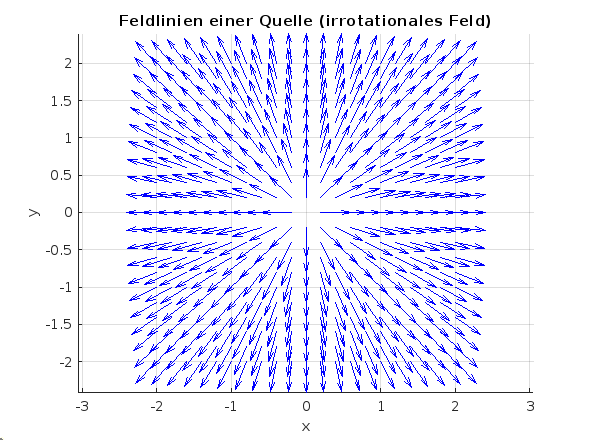
\includegraphics[width=0.7\textwidth]{papers/helmholtz/images/Quelle.png}
\caption{Quellenmuster im irrotationalen Feldanteil}
\label{fig:quelle}
\end{figure}
 
\begin{figure}
\centering
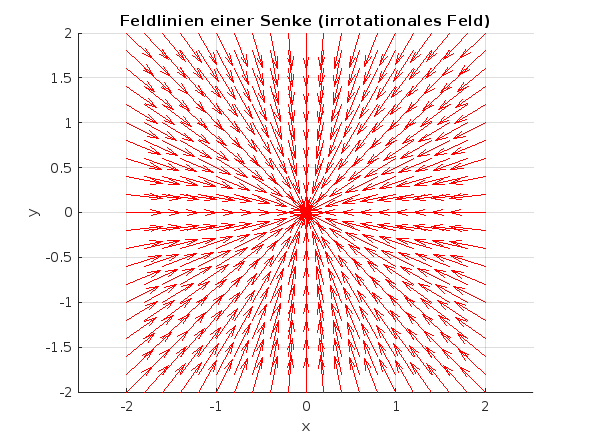
\includegraphics[width=0.7\textwidth]{papers/helmholtz/images/Senke.png}
\caption{Senkenmuster im irrotationalen Feldanteil}
\label{fig:senke}
\end{figure}
 
\item Der solenoidale Anteil bildet Wirbelfelder mit geschlossenen Feldlinien, ähnlich einem Magnetfeld.
\end{itemize}
  
\begin{figure}
\centering
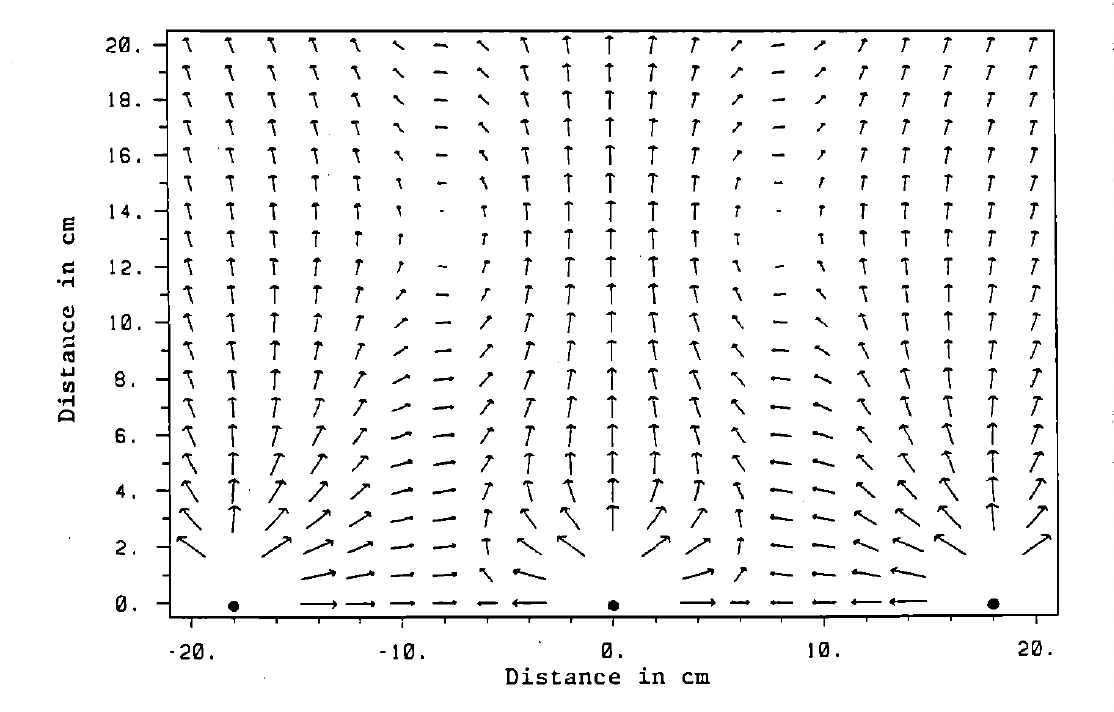
\includegraphics[scale=0.4]{papers/helmholtz/images/aktiveSchallintensitaet.png}
\caption{Visualisierung des aktiven Schallintensitätsfeldes für eine Anordnung von drei Punktquellen. Die Pfeile stellen die Vektoren der aktiven Intensität dar und zeigen die Richtung des zeitgemittelten Netto-Energieflusses. In der Nähe der Quellen ist die radial wegführende Energie zu erkennen, während in den Interferenzzonen komplexe Muster, einschliesslich der Bildung von Schallintensitätswirbeln, sichtbar werden (Abbildung aus \cite{helmholtz:paper}).}
\label{fig:aktive_intensitaet_3quellen}
\end{figure}
 
Die Visualisierung der Feldmuster erlaubt eine intuitive Interpretation von Schallfeldern:
 
\begin{itemize}
\item in Bereiche mit starker aktiver Intensität zeigen Energieausbreitung und -übertragung.
\item in Bereiche mit starker reaktiver Intensität zeigen Energieoszillation ohne Nettotransport, wie sie typischerweise im Nahfeld von Schallquellen oder bei stehenden Wellen auftritt.
\item Die räumliche Verteilung von Quellen, Senken und Wirbeln erlaubt Rückschlüsse auf die zugrundeliegenden Schallquellen und Reflexionsmuster. 

Abbildung \ref{fig:aktive_intensitaet_3quellen} verdeutlicht eindrücklich, wie die Interferenz von nur drei Quellen ausreicht, um solche komplexen Wirbelmuster zu erzeugen.
\end{itemize}
 
\noindent Diese Feldmuster sind besonders wichtig für die akustische Messtechnik, da sie eine visuelle Methode zur Identifikation von Schallquellen und zur Analyse von Energieflüssen in komplexen akustischen Feldern bieten.






\printbibliography[heading=subbibliography]
\end{refsection}
